%UCR-1: Inizializza sessione

\begin{figure}
\centering
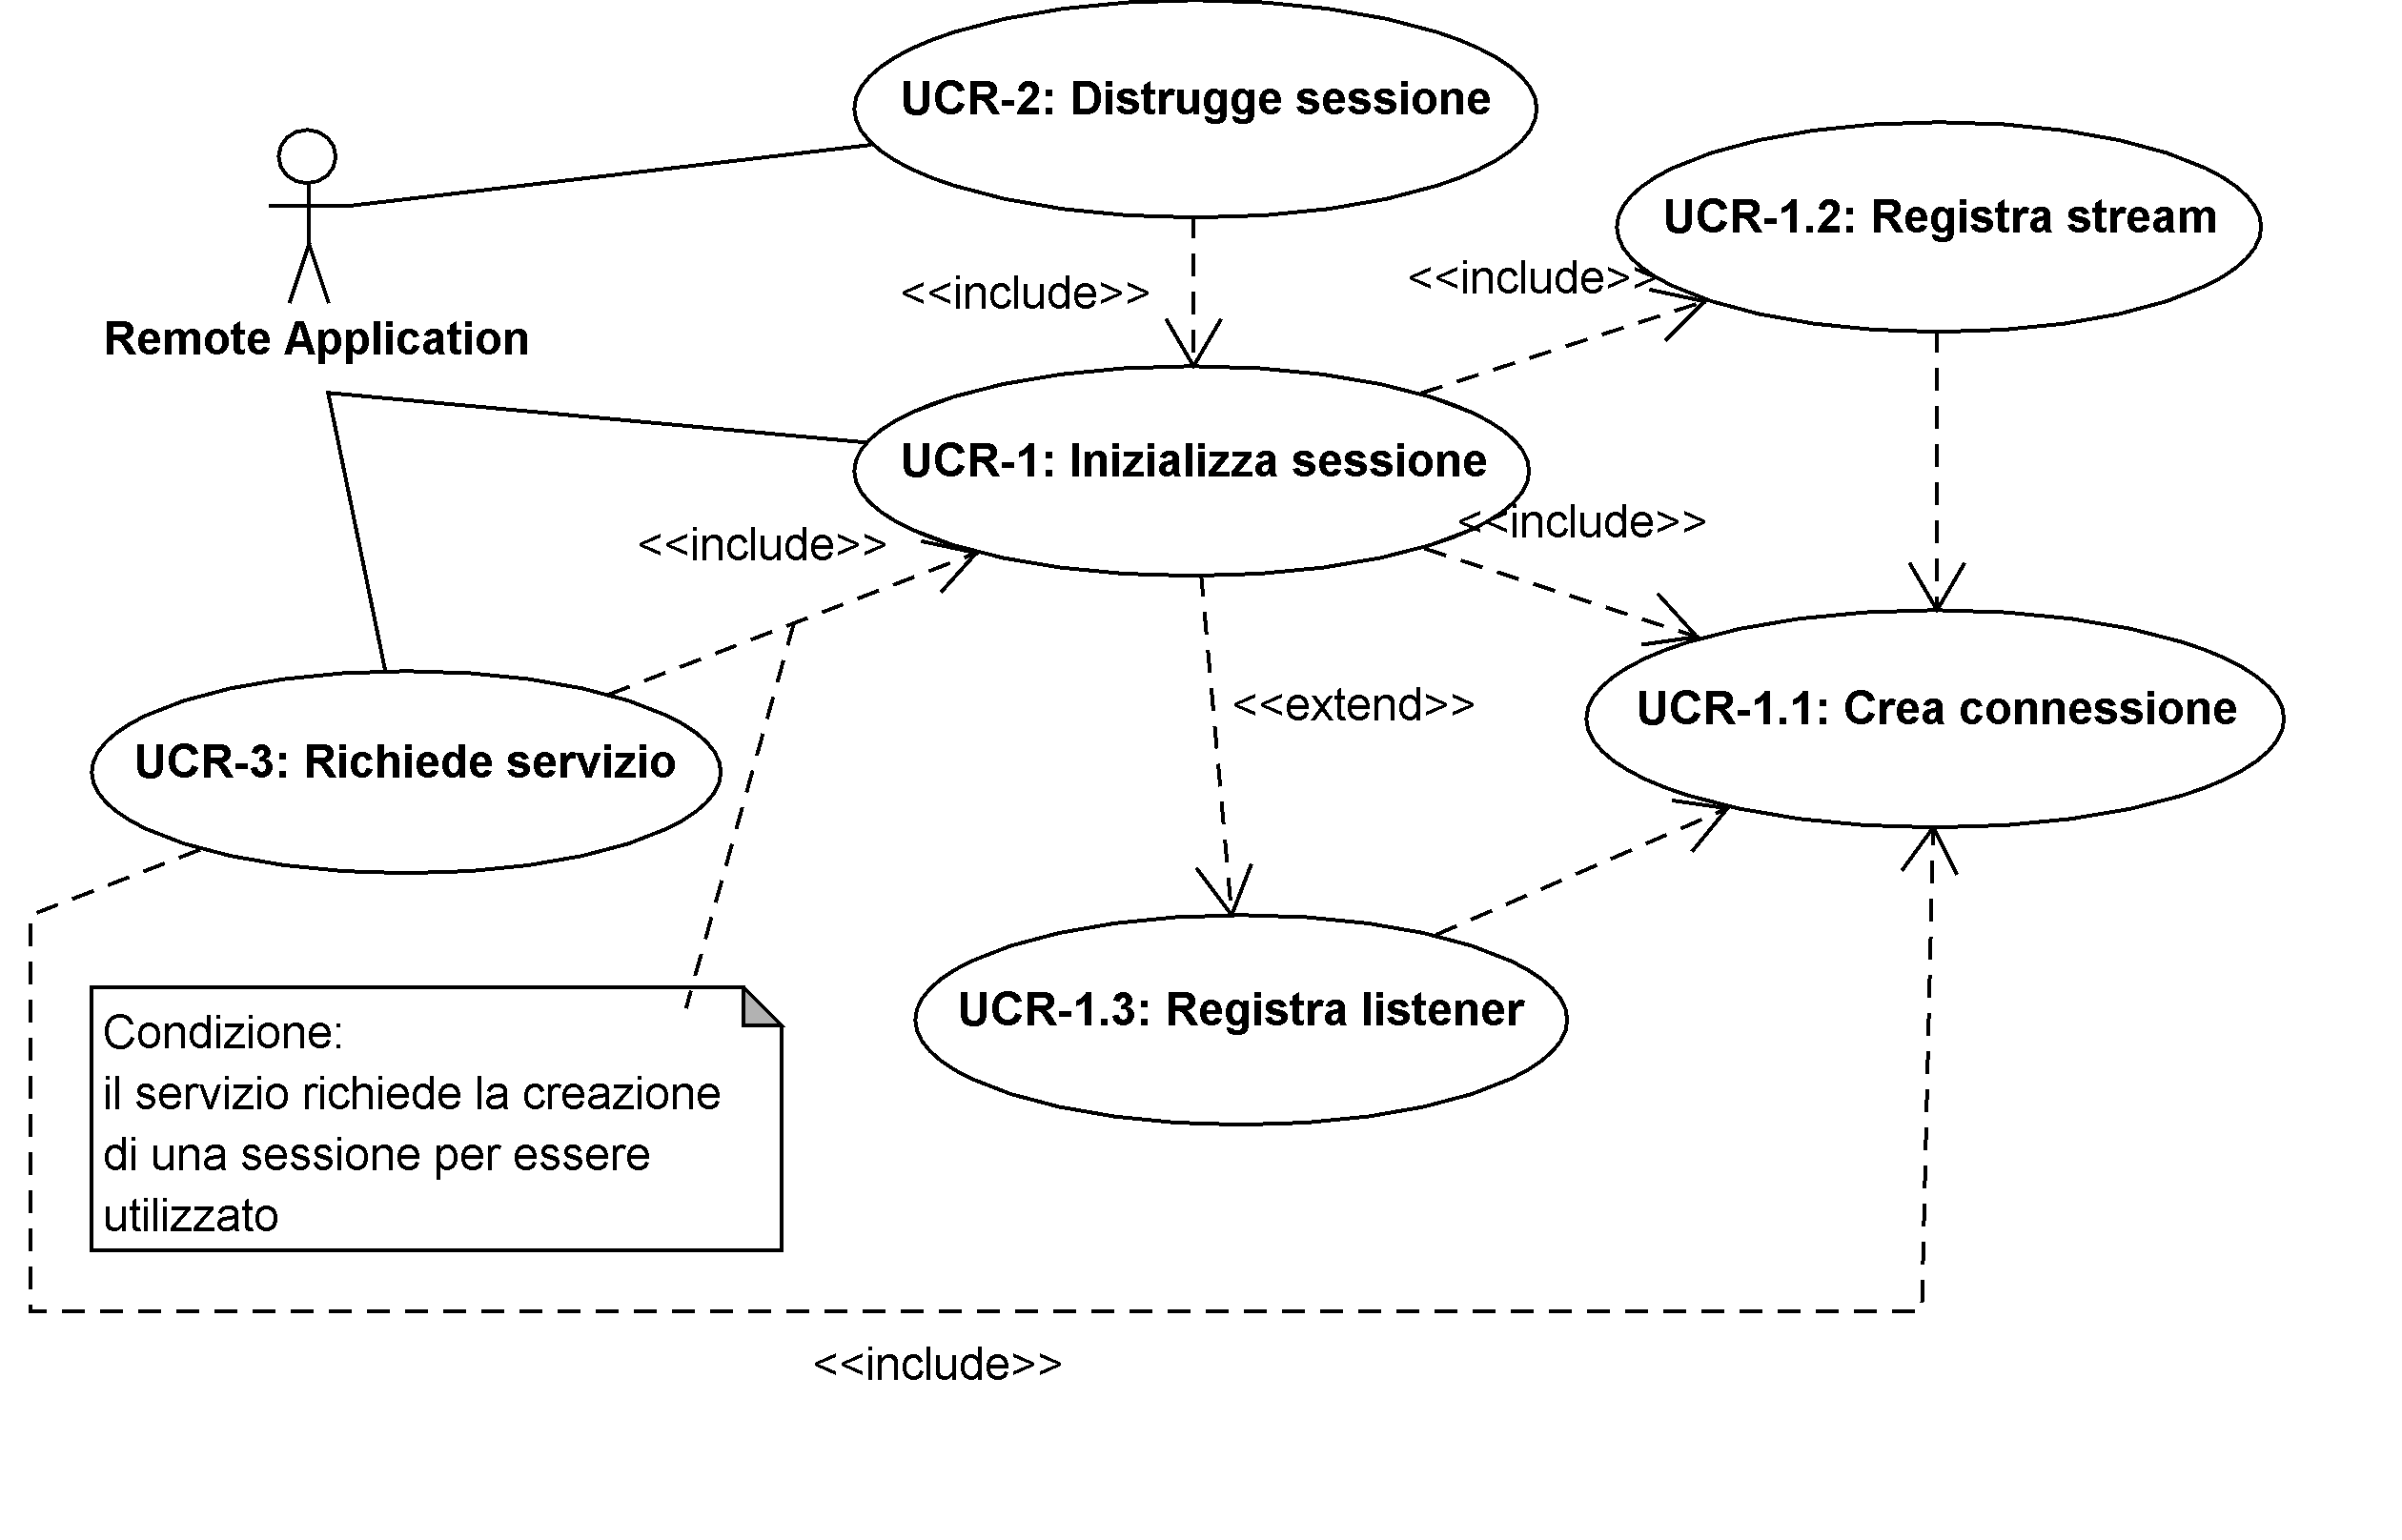
\includegraphics[width=1.1\textwidth]{Immagini/Capitolo2/UseCases/UCR-generale.png}
\caption{Diagramma dei casi d'uso UCR-1, UCR-2, UCR-3}\label{fig:uc-ucr-generale}
\end{figure}

Nel proseguo dei paragrafi relativi ai casi d'uso \emph{UCR}, il nome dell'attore \emph{Remote Application} verrà abbreviato con la sigla \emph{RA}.

\begin{itemize}
	\item \textbf{Attori:} Remote Application (\emph{RA})
	\item \textbf{Scopo e descrizione:} la RA deve avere la possibilità di inizializzare una sessione persistente con il software server che memorizzi le informazioni i dati che devono essere conservati fra richieste differenti
	\item \textbf{Pre-condizioni:} la RA ha conoscenza dei parametri di connessione relativi ad una istanza del software server
	\item \textbf{Post-condizioni:} la RA ottiene un codice univoco che identifica la sessione creata
	\item \textbf{Flusso principale degli eventi:}
		\begin{enumerate}
			\item la RA esegue una connessione con il server (si guardi il caso d'uso \emph{UCR-1.1})
			\item la RA richiede l'inizializzazione di una sessione
				\begin{itemize}
					\item la RA può fornire al server i parametri di connessione di uno stream (si guardi il caso d'uso \emph{UCR-1.2})
					\item la RA può fornire al server i parametri di connessione di un listener (si guardi il caso d'uso \emph{UCR-1.3})
				\end{itemize}
			\item la RA memorizza l'identificativo di sessione
		\end{enumerate}
	\item \textbf{Flusso alternativo:}
		\begin{enumerate}
			\setcounter{enumi}{1}
			\item se la RA non ottiene l'identificativo di sessione, lo scenario prosegue dal punto 1 del flusso principale
		\end{enumerate}
\end{itemize}


\paragraph{UCR-1.1: Crea connessione}

\begin{itemize}
	\item \textbf{Attori:} RA
	\item \textbf{Scopo e descrizione:} la RA deve avere la possibilità di stabilire una connessione con il server tramite protocollo XML-RPC
	\item \textbf{Pre-condizioni:} la RA ha conoscenza dei parametri di connessione relativi ad una istanza del software server
	\item \textbf{Post-condizioni:} la RA ha stabilito una connessione. Permette l'esecuzione dei casi d'uso \emph{UCR-1}, \emph{UCR-1.2}, \emph{UCR-1.3}, \emph{UCR-3}
	\item \textbf{Flusso principale degli eventi:}
		\begin{enumerate}
			\item la RA stabilisce una connessione seguendo le specifiche del protocollo XML-RPC
		\end{enumerate}
	\item \textbf{Flusso alternativo:}
		\begin{enumerate}
			\item se la connessione fallisce, la RA attiva un protocollo di gestione dell'errore (la definizione del protocollo è materia della RA)
		\end{enumerate}
\end{itemize}


\paragraph{UCR-1.2: Registra stream}

\begin{itemize}
	\item \textbf{Attori:} RA
	\item \textbf{Scopo e descrizione:} la RA deve essere in grado di registrare uno stream remoto utilizzabile dal software server 
	\item \textbf{Pre-condizioni:} la RA ha eseguito con successo il caso d'uso \emph{UCR-1.1}
	\item \textbf{Post-condizioni:} il software server può utilizzare lo stream remoto come sostituto di uno locale. Permette l'esecuzione dei casi d'uso \emph{UCC-1.2.1} e \emph{UCC-1.2.2} anche per l'attore RA
	\item \textbf{Flusso principale degli eventi:}
		\begin{enumerate}
			\item la RA fornisce al software server i parametri di connessione di uno stream remoto
			\item la RA indica:
				\begin{enumerate}
					\item indirizzo e porta di connessione dello stream
					\item nome dello stream remoto
					\item nome dello stream per il software server
					\item un codice di controllo
				\end{enumerate}
			\item la RA riceve un segnale di conferma all'indirizzo indicato usando i parametri forniti
			\item lo stream remoto è indicato come sostituto di uno stream locale
		\end{enumerate}
	\item \textbf{Flusso alternativo:}
		\begin{enumerate}
			\setcounter{enumi}{2}
			\item se la RA non ottiene un segnale di conferma dopo un tempo massimo stabilito, la RA attiva un protocollo di gestione dell'errore (la definizione del protocollo è materia della RA)
			\item lo stream remoto viene ignorato
		\end{enumerate}
\end{itemize}


\paragraph{UCR-1.3: Registra listener}

\begin{itemize}
	\item \textbf{Attori:} RA
	\item \textbf{Scopo e descrizione:} la RA deve essere in grado di registrare un listener remoto utilizzabile dal software server 
	\item \textbf{Pre-condizioni:} la RA ha eseguito con successo il caso d'uso \emph{UCR-1.1}
	\item \textbf{Post-condizioni:} il software server può utilizzare il listener remoto come sostituto di uno locale. Permette l'esecuzione del caso d'uso \emph{UCC-1.2.3} anche per l'attore RA
	\item \textbf{Flusso principale degli eventi:}
		\begin{enumerate}
			\item la RA fornisce al software server i parametri di connessione di un listener remoto
			\item la RA indica:
				\begin{enumerate}
					\item indirizzo e porta di connessione del listener
					\item nome del listener remoto
					\item nome del listener per il software server
					\item il nome degli eventi per i quali registrare il listener
					\item un codice di controllo
				\end{enumerate}
			\item la RA riceve un segnale di conferma all'indirizzo indicato usando i parametri forniti
			\item il listener remoto è indicato come sostituto di uno locale
		\end{enumerate}
	\item \textbf{Flusso alternativo:}
		\begin{enumerate}
			\setcounter{enumi}{2}
			\item se la RA non ottiene un segnale di conferma dopo un tempo massimo stabilito, la RA attiva un protocollo di gestione dell'errore (la definizione del protocollo è materia della RA)
			\item il listener remoto viene ignorato
		\end{enumerate}
\end{itemize}



